\chapter{The improved SimpleSTORM algorithm}
STORM data from different cells or structures show many different features: there can be clusters of fluorophores with a high density of spots, areas with low density, variable background in space and time, beads can be present or absent.\newline
This section describes how the algorithm processes the data sets and how it is possible to find good settings that will work for all kind of input data. The changes and improvements over the previous version are described and discussed. The new GUI design and the new features are introduced.\newline
All real world images shown in this thesis were acquired from members of Prof. Dr. Mike Heilemanns group.


\section*{Import and processing}
STORM data usually has a size of around 3 gigabytes. However larger data sets are possible too, making it necessary to work on smaller parts of the data, instead putting the whole dataset into memory. This is done using chunks of a user defined size. The data is processed chunkwise, and the processing of the frames of each chunk can be parallelized. This parallelization is possible because the signals in each frame are considered to be independent from each other. There is a dependency between different chunks. The mean values of several chunks are used to estimate the background. Therefore a certain number of mean values has to be stored in memory.

\section{Workflow}
\subsection{Choosing parameters}
Initially the user has the option to set all important parameters. If no parameter is set the default ones are used and will give a good result because all crucial parameters are either determined from the data or set to reasonable values that work for every data set. The goal of the default parameters is to give a good result with no adjustment. This means parameters are chosen to produce almost 100 \% precision. It is assumed that the loss of some points that are not detected using this conservative setting will not affect the final result as much as a lower precision would.
\subsection{Estimating camera gain and offset}
First the application checks for a file containing settings for gain and offset from an earlier run. If this is not the case new parameters are estimated based on the first part of the data; usually 200 frames are sufficient.\newline
A set of 2000 pixels is chosen by their mean intensity with respect to time. Therefore the mean intensity range is divided in 2000 bins. For each bin one pixel with the appropriate mean is selected. For faster computation the mean is not calculated over all frames but only over a certain, user defined, number. The goal is to get pixels with the whole range of mean intensities, good representatives from the darkest background pixel to the brightest beads.\newline 
The method described in section \ref{skellam1} is used to estimate the gain factor, based on the preselected points. The variances of the pixels are computed based on the first part of the data.
Each dataset is three-dimensional, where time is the third
dimension. Therefore mean $\mu$ and variance $\sigma^2$, in time, can be calculated from
the data for each pixel individually
\begin{align}
	\mu(i,j) & = \frac{\Sigma_t(I_t(i,j)(i,j))}{n}\\
	\sigma^2 & = \frac{\Sigma_t(\mu(i,j)-(I_t(i,j)))^2}{n-1}
\end{align} 
$I_t(i,j)$ describes the intensity of the pixel of frame $t$ at position $i,j$.
To determine the gain factor the variances $\sigma^2$ for each pixel are plotted over the mean
intensities. A straight line can be fitted, and its slope gives the gain
factor, the $x$-intersection gives the offset.\newline 
Figure \ref{skellamplot} shows the scatter plot for the selected points and the fitted line. The data is taken from a real world data set. The red dots result from pixels that have a constant mean intensity over time. They are either dark the whole time, these are the dots on the left or they are beads and show signal in every frame. The blue dots result from pixels that are sometimes covered by a PSF. This blinking has much stronger influence on the variance than for the pixels mean values. This is the reason why this points are clustered on the lower end of the mean intensities. \newline
For a robust estimation of the straight line a RANSAC (random sample consensus) algorithm is used. It is described in section \ref{ransacdescr}. 

\begin{figure}
\centering
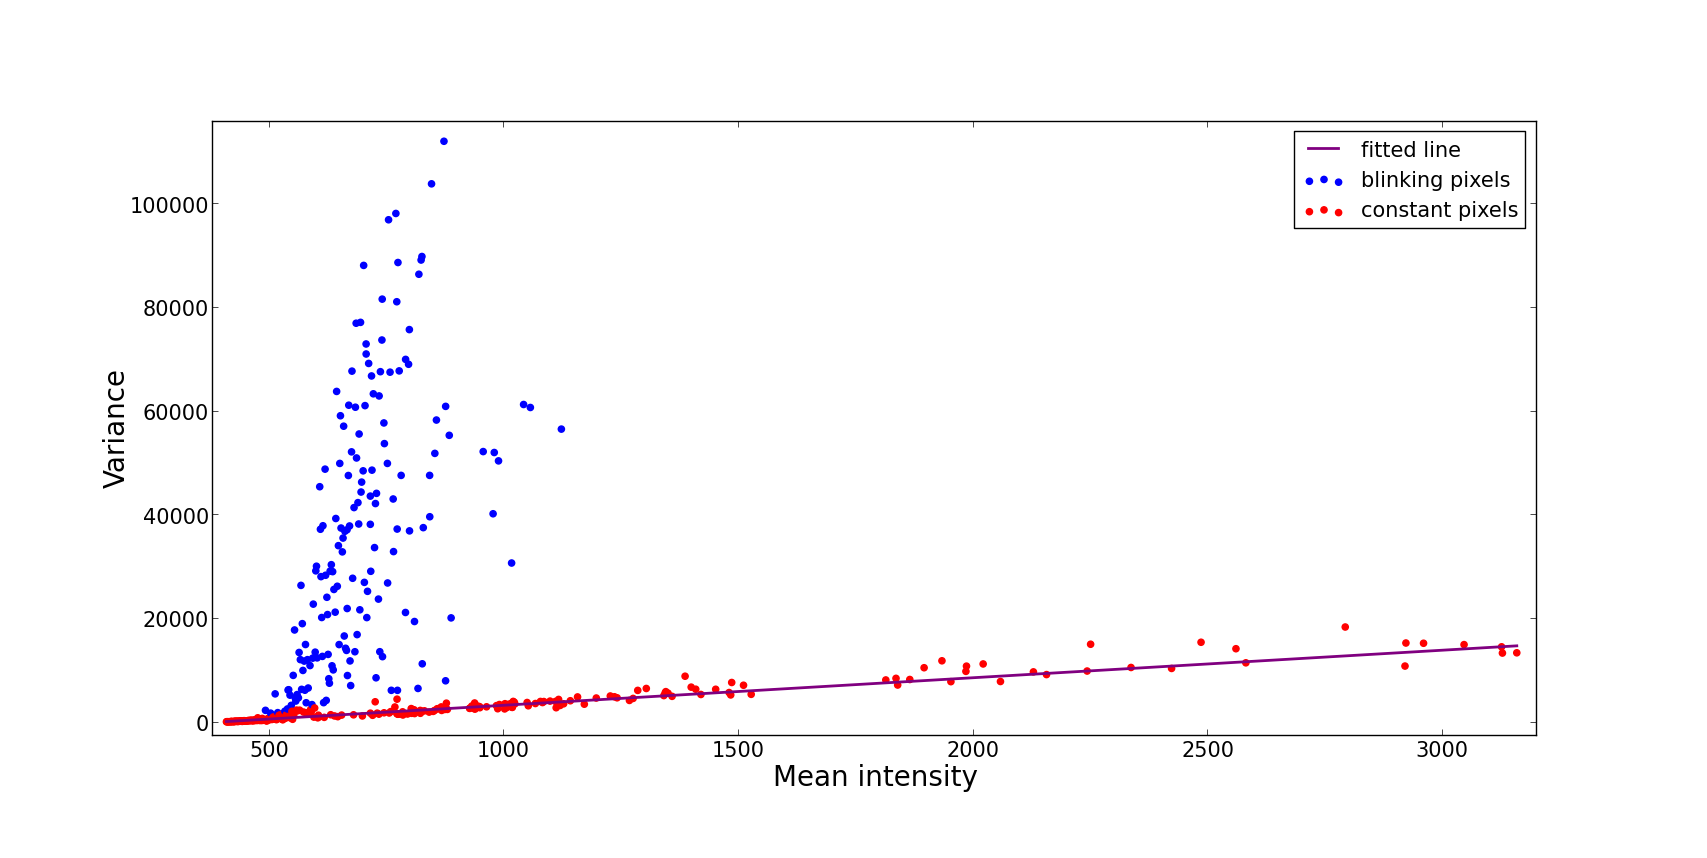
\includegraphics[width = 0.99\textwidth]{pictures/skellamplot.png}
	\caption{Scatter plot for the preselected points. Blue points result from pixels that show at least once a higher intensity caused by a fluorophore. The red dots are used to determine the gain and offset.}
	\label{skellamplot}
\end{figure}
\subsection{Recursively adjusting gain and offset}
After the estimation of gain factor and offset, the transformations described in section \ref{trafoPoiss} and section \ref{trafoAnscombe} are applied and the background is subtracted.\newline
Due to the Anscombe transformation, the background pixels of the image should only vary around a mean intensity of zero with a variance of one. Therefore, a histogram of the pixel intensities is created. After background subtraction, the background pixels should contribute only to the lower intensities in the histogram. A Gaussian function is fitted to the histogram's values. This is done under the assumptions that there is much more background in the image than signal, or that the intensities coming from signals are distributed over a larger range, so the Gaussian for the background intensity distribution can be fitted correctly.\newline


If the estimated value for the variance is too far from one, the originally estimated gain factor is corrected and applied, and the fit is done again (compare section \ref{checkGain}). This is done until the background variance converges within a small threshold or the maximal number of iterations is reached. In this case the initial gain factor will be used and a warning will be shown on the screen.\newline
It might be that the correction of the gain factor gets trapped duo to overshooting. In that case the estimated background variances oscillate around one. If this is the case the mean gain factor from the last two corrections is used.
\subsection{Estimating the width of the point spread function}
An inverse Anscombe transformation (equation \ref{invAnsc}) is applied to the data. This is necessary because the Anscombe transformation increases the point spread functions width, depending on the intensity of the point spread function. This is shown in section \ref{PSF}.\newline  
For 20 local maxima of a certain, user defined, number of frames the square of the Fourier transformation off each region of interest around the chosen local maxima is calculated. This squared Fourier transformations are then averaged. The result is called the mean power spectrum. It can be used to estimate the variance of the point spread function of the signal. A two dimensional Gaussian function's Fourier transform is again a Gaussian but with inverse variance. This relation is used to determine the variance of the point spread function in the spatial domain, using the fit parameter for the variance in the frequency domain.\newline
The script for fitting the two dimensional Gaussian function was implemented by Ilia Kats.
\subsection{Processing the data}
\subsubsection{Import Data}
Storm data sets can consist of several thousand frames with resolutions up to one megapixel per frame. This size makes it necessary to break the data into smaller parts, otherwise it could be larger than the RAM of an ordinary machine. Because of the background estimation, it is not possible to process every frame completely independently as it was in the older version of this software (\cite{MAJoachim}). 
%For the hdf5 data format it is faster to load a larger consecutive part of the dataset into memory instead of loading each frame.
\newline
This algorithm uses chunks of user defined size. There are some limitations to the chunk size that are discussed later. The data set is split into parts of equal size in the $x$- and $y$-dimensions and independently also in the $t$-dimension. If this partition does not fit at the edge of the data set, the last chunks will be smaller.\newline
The data is transformed to be Poisson distributed, then the Anscombe transform is applied which gives background intensities with unit variance.\newline
The implementation of the workflow using chunks was done by Ilia Kats.
\subsubsection{Background estimation} \label{bgestimation}
For each chunk, the median of the Anscombe transformed data is determined to get a robust estimate of the background value for this chunk. 
B-spline interpolation, implemented in vigra (\cite{vigra}), is used to get interpolated values for the full resolution of the current frames. For this interpolation, three chunks in both the spatial and the temporal domain have to be available. Therefore the maximal chunk size into $t$-dimension must not be larger than a third of the total stack size, the same holds for the chunk size in $x$ and $y$ direction which must not exceed the spatial resolution of the image stack. These values are checked automatically and changed if necessary.\newline
The interpolated background is then subtracted from the transformed data to give background pixels with zero mean and unit variance, both in $xy$- and in $t$-dimension. Figure \ref{removedBG} shows an frame with variable background before and after background subtraction.
\begin{figure}
\subfloat[Original image]{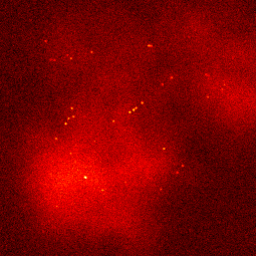
\includegraphics[width = 0.485\textwidth]{pictures/Tubulin2OrigFrame50Color.png}}\hfill
\subfloat[image after background subtraction]{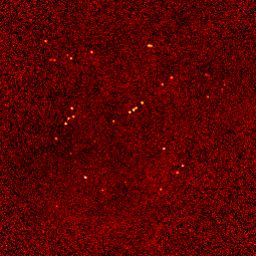
\includegraphics[width = 0.485\textwidth]{pictures/Tubulin2normalprocessFrame50Color.png}}
	\caption{Effect of background subtraction on an inhomogeneous background. For the human eye no more points are visible but for computers it is much easier to find the bright spots in the background subtracted image, because a global threshold can be applied or as in the case of SimpleSTORM the probabilistic model can be tested.}
	\label{removedBG}	
\end{figure}
\subsubsection{Create mask for background suppression}
With the given $p$-value from the settings, a global threshold can be determined, because inhomogeneities of background intensities have been removed. The threshold value is that intensity 
for which the integral over the probability density function of a Gaussian distribution with zero mean and unit variance gives $1-p$. It is that intensity for which it is less likely than $p$ to occur. This threshold is possible because the background intensities follow a Gaussian distribution, with known mean and variance, after all transformations applied.\newline
The threshold is applied to the current frame and a binary mask is stored. For the reason that it is possible for bright background pixels to exceed the threshold, the connected components of the mask are calculated. Pixels that belong to connected components with too few members are discarded. The idea behind using connected components is, that there is a probability for a background pixel to be brighter than the threshold, but it is unlikely that two neighboring pixels exceed the threshold in the same frame and even more unlikely that three of them do so. Therefore the number of pixels necessary for keeping a connected component is set to a minimum of three. If the width of the point spread function is very large the critical size of the connected components can be set depending on the PSF width. But to suppress background pixels efficiently the number of pixels in a connected component has to be larger than two.
\subsubsection{Filtering data and finding maxima}
To improve the accuracy of the spot detection, the transformed signal is convolved with a two dimensional Gaussian function with the previously determined or user-set width. The convolved image will further be used to find the maxima. All local maxima in the frame are detected. Each maximum found is tested to be covered by the mask or discarded otherwise. A region of interest around the remaining maxima is interpolated to a higher resolution. The interpolated region is searched for local maxima once again. These maxima will be detected with super resolution.\\
To determine the signal-to-noise ratio, the unfiltered and uninterpolated pixel intensity is used.
This maxima detection was already implemented by Joachim Schleicher (\cite{MAJoachim}).
\subsubsection{Quality control for detections}
Sometimes, especially in data sets with a high density of spots, two spots are near enough that their point spread functions overlap. It may happen that instead of two maxima only one maximum will be detected between the true ones, as can be seen in Figure \ref{betterthansimplestorm}. This leads to large errors in the localization. To avoid this a threshold for the asymmetry of the spots can be set.\newline
The calculation of the asymmetry was already implemented by Joachim Schleicher \cite{MAJoachim}.


\section{Comparison with older version of the SimpleStorm algorithm}
\subsection{Adjustable filter width} \label{sectionFilterisEvil}
If two or more point spread functions (PSF) overlap, applying a smoothing filter can lead to the merging of point spread functions. This merging becomes a problem if the two distinct maxima of the original unsmoothed PSFs form a new maxima in between. This leads to just one detection somewhere between the true maxima. The number of merging PSFs increases with greater filter widths. For high density data it might be better to use a filter with smaller width and therefore less accuracy, but fewer merged PSFs. In total this might give a better result depending on the number of incorrectly merged PSFs. This is the reason why filtering was changed to use just a Gaussian filter instead of the Wiener filter originally used. 
The effect of the smaller filter width can be seen in Figure \ref{betterthansimplestorm}. The red crosses indicate detections found by the new SimpleSTORM version, the green crosses show the estimated positions found by the previous version of SimpleSTORM, and the white x marks the true location. The predictions by the newer version are not perfect but better than the predictions of the older version. The scores that can be seen in Table \ref{tabelbetterthansimplestorm} are calculated like as described in section \ref{measuresISBI}. Both results have almost the same accuracy, but differ in the scores. There are two effects related to the accuracy canceling each other out. Fewer merged PSFs increase the accuracy, but the positive effect of filtering with the appropriate filter, as shown in Figure \ref{accplot2} or in Figure \ref{matchedFilter1}, is lost.

\begin{table}
\caption{Comparison of results created using almost no smoothing or Wiener filter on high density data. Although the accuracy is almost the same, the number of detections and the scores are higher for the unsmoothed data. For the evaluation software from the \cite{challenge} were used.}
\begin{tabular}{l|llllll}
&intersections&Jaccard&F-Score&Precision&Recall&RMSE\\ \hline
Gaussian filter, $\sigma$ = 0.01& 16955&19.99&33.26&81.10&20.92&27.21\\
Wiener filter& 14480&17.06&29.15&79.19&17.87&27.28
\end{tabular} \label{tabelbetterthansimplestorm}

\end{table}


\begin{figure}
\subfloat[Advanced setting widget]{
\includegraphics[width = 0.485\textwidth]{pictures/betterthanSimplestorm1.png}}\hfill
\subfloat[Easy setting widget]{
\includegraphics[width = 0.485\textwidth]{pictures/betterthanSimplestorm2.png}}
	\caption{This pictures show the effect of a smaller filter width. The red crosses show detections found with a filter width of 0.01, the green crosses the results using a Wiener filter. The white x marks the ground truth.}
	\label{betterthansimplestorm}	
\end{figure}

\subsection{False positive suppression}
In the previous version the background was determined by first estimating a baseline. The minimum of the current frame was taken as the baseline. It was subtracted from the image and the result was smoothed with a Gaussian filter of width ten. The smoothed image was subtracted from the original image to give a background free image. This works fine for subtracting background with variations larger than the filters width, but the resulting intensities do not contain any information about the variability of the background intensities.\newline
If, for example, the resulting intensity, after background subtraction, is five. This can either mean it is most likely signal, given that the variance of the background in the original image was very small, or it can mean nothing, if the variance of the original background pixels were 20. In the latter case the probability that the difference of five between the original image and the smoothed one has a high chance to result from the background variation.\newline
In the older version of SimpleSTORM the intensity of a candidate, considered to be a signal, was checked 
whether its intensity after the background subtraction was higher than the estimated background value at the maximums position minus the baseline. This works for homogeneous background intensities but fails if the baseline, gets a small value from a region with small background values and is applied to a bright region. In that case the intensity of the estimated background gives high values at the maximums position but only a small value is subtracted. This results in discarding many maxima in regions of bright background as in Figure \ref{bgmakesitbad}.
The old version of SimpleSTORM only finds about 8000 spots while the new version finds more than 44000 on a test data set with high background variance. Using the new background suppression results in a reconstructed image that shows the reconstructed structures in a better way.

\begin{figure}
\subfloat[Typical frame showing variable background intensities]{
\includegraphics[width = 0.3\textwidth]{pictures/Tubulin2OrigFrame50.png}}\hfill
\subfloat[Result old SimpleSTORM]{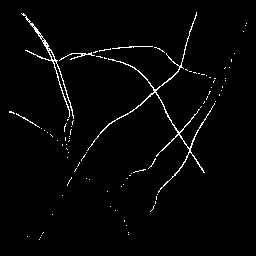
\includegraphics[width = 0.30\textwidth]{pictures/Tubulin2factor1OldSimpleSTORM.png}}\hfill	
\subfloat[Result new SimpleSTORM]{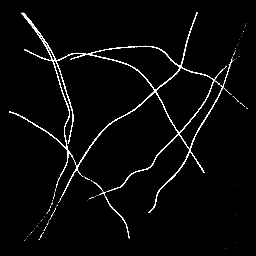
\includegraphics[width = 0.3\textwidth]{pictures/Tubulin2factor1.png}}

\caption{This pictures show the drawback of the old background treatment. On the left a typical frame with variable background is shown. The old version of SimpleSTORM discards many detections in the regions of high background intensity. The new SimpleSTORM software discards detections based on their signal-to-noise ratio and is less affected by variable background.}
\label{bgmakesitbad}	

\end{figure}

The great advantage of the newer version of SimpleStorm is its model for the background. For each pixel, the probability to be signal can be determined based on its signal-to-noise ratio. Using the number of connected components of each cluster, false positive detections caused by bright background pixels can be suppressed.

\subsection{Comparable results based on the signal-to-noise ratio}
The accuracy of the maxima detection relies on the signal-to-noise ratio (SNR). With a given SNR the correct standard deviation of the localization error can be used for further calculations (the calculation for the localization error is done in section \ref{detectionError}). This is not possible if only intensities are saved because without information about the backgrounds variance the reliability of the detection can't be estimated.\newline
Saving the signal-to-noise ratio also enables to compare results from either different cameras or different settings or a different environment that might lead to a higher background variability.  


\section{New graphical user interface (GUI)}
\subsection{Input widget}
The new GUI for SimpleStorm was designed to integrate its many new features. Figure \ref{guiWidgets} shows this new design. \newline
There are three categories of parameters. The first category specifies which upsampling factor will be used, the width of the pixels in nanometers of the input data, the reconstruction resolution, the number of frames that are used to estimate the camera parameters and the PSFs width and sensitivity of the algorithm. The first three parameters are general information that depend on the capturing process of the data and the desired upsampling factor. Two of them must be set and the third is calculated automatically.\newline
The most challenging parameters of this section are the alpha value, which sets the sensitivity for false detections and the number of frames used for estimation of the camera parameters and the PSF. For these values the default setting are set to work well with any data sets. \newline
The next category of parameters defines the width of the region of interest (ROI) for the estimation of the point spread function and the chunk sizes in spatial and temporal dimension can be set. There are two different ways to set these parameters (see Figure \ref{guiSettings}). One is to give values for all parameters. This is difficult without understanding the influence of these parameters on the algorithm. Therefore there is also a second way to set this parameters. The user should know some properties of the data that shall be processed, such as: is the spot density high or low? Is there variable background in time and space? Depending on the sliders' positions, the best parameters are set automatically. How this is done will be described in section \ref{easyParam}. With this second option the user can process his or her data, treating variable background or dense data without deep insight or understanding of the algorithms.\newline
The last category of parameters describes the camera gain and offset, the width of the signals point spread function, and a prefactor that can be used to alter the estimated gain. 
\begin{figure}
\subfloat[Easy setting widget]{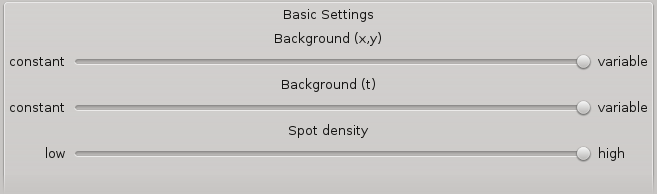
\includegraphics[width = 0.465\textwidth]{pictures/basicSettingsGui1.png}}
\subfloat[Advanced setting widget]{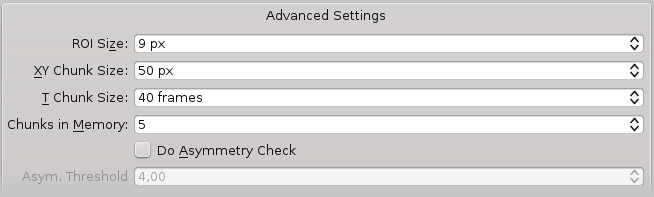
\includegraphics[width = 0.465\textwidth]{pictures/advancedSettingsGui.png}}\hfill
	\caption{There are two different ways to set the parameters for the algorithm. On the right the standard way of setting parameters can be seen. On the left, there are sliders that can be adjusted between the extremes. The program sets the value for the parameters in a way to produce the best results for the selected attributes of the data set.}
	\label{guiSettings}	
\end{figure}
\subsection{Result widget}
After the run button at the lower left edge of the input widget is pressed, a new tab opens. In this widget the reconstructed image is shown. At the bottom there is a progress bar that displays the current processing step and its progress. Buttons to zoom in and out or to fit the displayed image into the window are located in the lower part of the result widget. On the lower right there is the stop/save button. It either stops the program if it is still running or opens a dialog to save the result image and the coordinates of the detection if the program has already been stopped.\newline
The GUI was mainly designed by Ilia Kats.

\begin{figure}
\subfloat[Input widget]{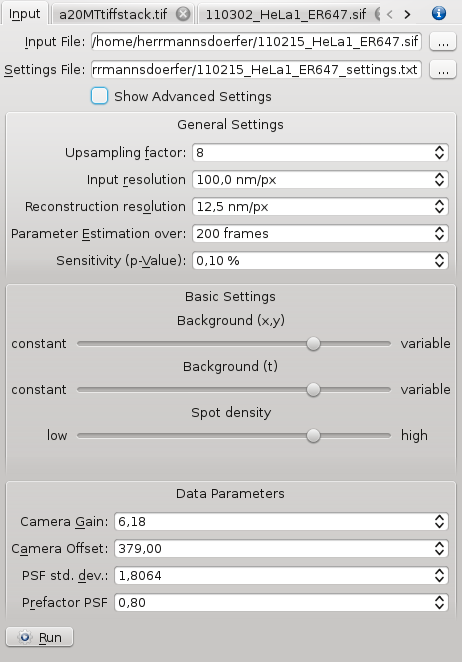
\includegraphics[width = 0.405\textwidth]{pictures/InputWidget.png}}\hfill
\subfloat[Result widget]{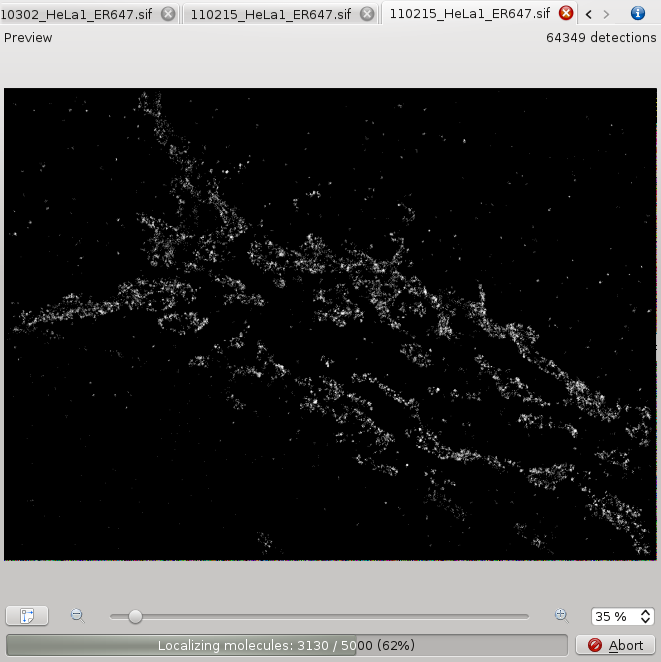
\includegraphics[width = 0.575\textwidth]{pictures/ResultWidget.png}}
	\caption{The new GUI. On the left is the window for selecting input file and parameters. On the right is the result widget showing the processing of a data set in progress.}
	\label{guiWidgets}	
\end{figure}

\subsection{Easy parameter selection}\label{easyParam}
As mentioned above the easy setting widget makes it easy to set reasonable parameters without knowing their influence on the algorithms.\newline
The background sliders have direct influence of the corresponding chunk size. A more constant background gives better results with larger chunks. This is because the median of all pixels in a chunk is used to estimate the mean value of the background. For the estimation of this relation between the median and the mean $\lambda$ of a Poisson distribution, described in equation \ref{meanMedianPoiss}, is used.
Because of the high mean values for $\lambda$ the last summand can be dropped.
This estimation works only if the chunks contain more background pixels than signal, otherwise the mean value will be overestimated. With large chunks this assumption is satisfied. But the smaller the chunk size, the more likely it is that a cluster of points lies in the chunk, and the values of the median are too high. On the other hand, the chunk sizes should be within the range of the changes in background. The best chunksize is therefore in the range of the variable background. The slider position sets the chunk sizes linearly to a value that lies in between the smallest and the largest chunk size possible for the data set.\newline
The minimal possible chunk size is 3 pixels. The largest chunk size possible is half of the shorter border in $x$ and $y$ dimension and the number of frames over which the parameters are estimated divided by the number of chunks in memory in $t$ dimension. These restrictions to the maximal chunk size result from the spline interpolation as described in section \ref{bgestimation}.\newline 
In general, the denser the dataset is, the more likely it is that two neighboring PSFs are merged due to the filtering, as shown in section \ref{sectionFilterisEvil}. There are two ways to avoid inaccurate detections that result from merged PSFs. One is less filtering, to avoid merges, the second one is checking the symmetry of the detected spots. Merged spots become more and more asymmetric the further the two true centers of the PSFs lie apart from each other. A high asymmetry is a good indicator for a detected spot with low accuracy.
The spot density influences the prefactor for the estimated sigma and the value for the asymmetry checks. It sets the threshold for the asymmetry in the same way the sliders for background work, within appropriate limits, with higher values for the asymmetry threshold for less dense data sets. Also, the prefactor is set to values between 1 for sparse data and zero for dense data.